
\subsection{Expert Transformer}\label{sec:expert-transformer}

We introduce the design choices in Transformer for \model, including the patching, positional embedding, and attention strategies for handling the text-video data effectively and efficiently. 

\paragraph{Patchify.}
The 3D causal VAE encodes a video latent of shape $T \times H \times W \times C$, where $T$ represents the number of frames, $H$ and $W$ represent the height and width of each frame, $C$ represents the channel number, respectively.
The video latents are then patchified, generating sequence $z_{\text{vision}}$ of length $\frac{T}{q}\cdot \frac{H}{p} \cdot \frac{W}{p}$. 
When $q > 1$, we repeat the first frame of videos and images at the beginning of the sequence to enable joint training of images and videos.
% Note that, we do not patchify along the temporal dimension in order to enable joint training of images and videos.

\paragraph{3D-RoPE.}
Rotary Position Embedding (RoPE)~\citep{su2024roformer} is a relative positional encoding that has been demonstrated to capture inter-token relationships effectively in LLMs, particularly excelling in modeling long sequences. 
To adapt to video data, we extend the original RoPE to 3D-RoPE. 
Each latent in the video tensor can be represented by a 3D coordinate $(x, y, t)$.
We independently apply 1D-RoPE to each dimension of the coordinates, each occupying $3/8$, $3/8$, and $2/8$ of the hidden states' channel. 
The resulting encoding is then concatenated along the channel dimension to obtain the final 3D-RoPE encoding. 

% We empirically examine the use of RoPE. 
% Figure~\ref{fig:subfigures} (a)shows the comparison between 3D RoPE and sinusoidal absolute position encoding. 
% We can observe that the loss curve using 3D RoPE converges significantly faster than that with sinusoidal encoding. 
% We further compare the use of 3D RoPE alone against the combination of 3D RoPE and learnable absolute position embedding. 
% Figure~\ref{fig:subfigures} (b) indicates that the loss curves of both methods converge almost identically. 
% Therefore, we choose to use 3D RoPE alone for simplicity. 


%\section{Ablation}
% \begin{figure}[h]
%     \centering
%     \begin{subfigure}[b]{0.46\textwidth}
%         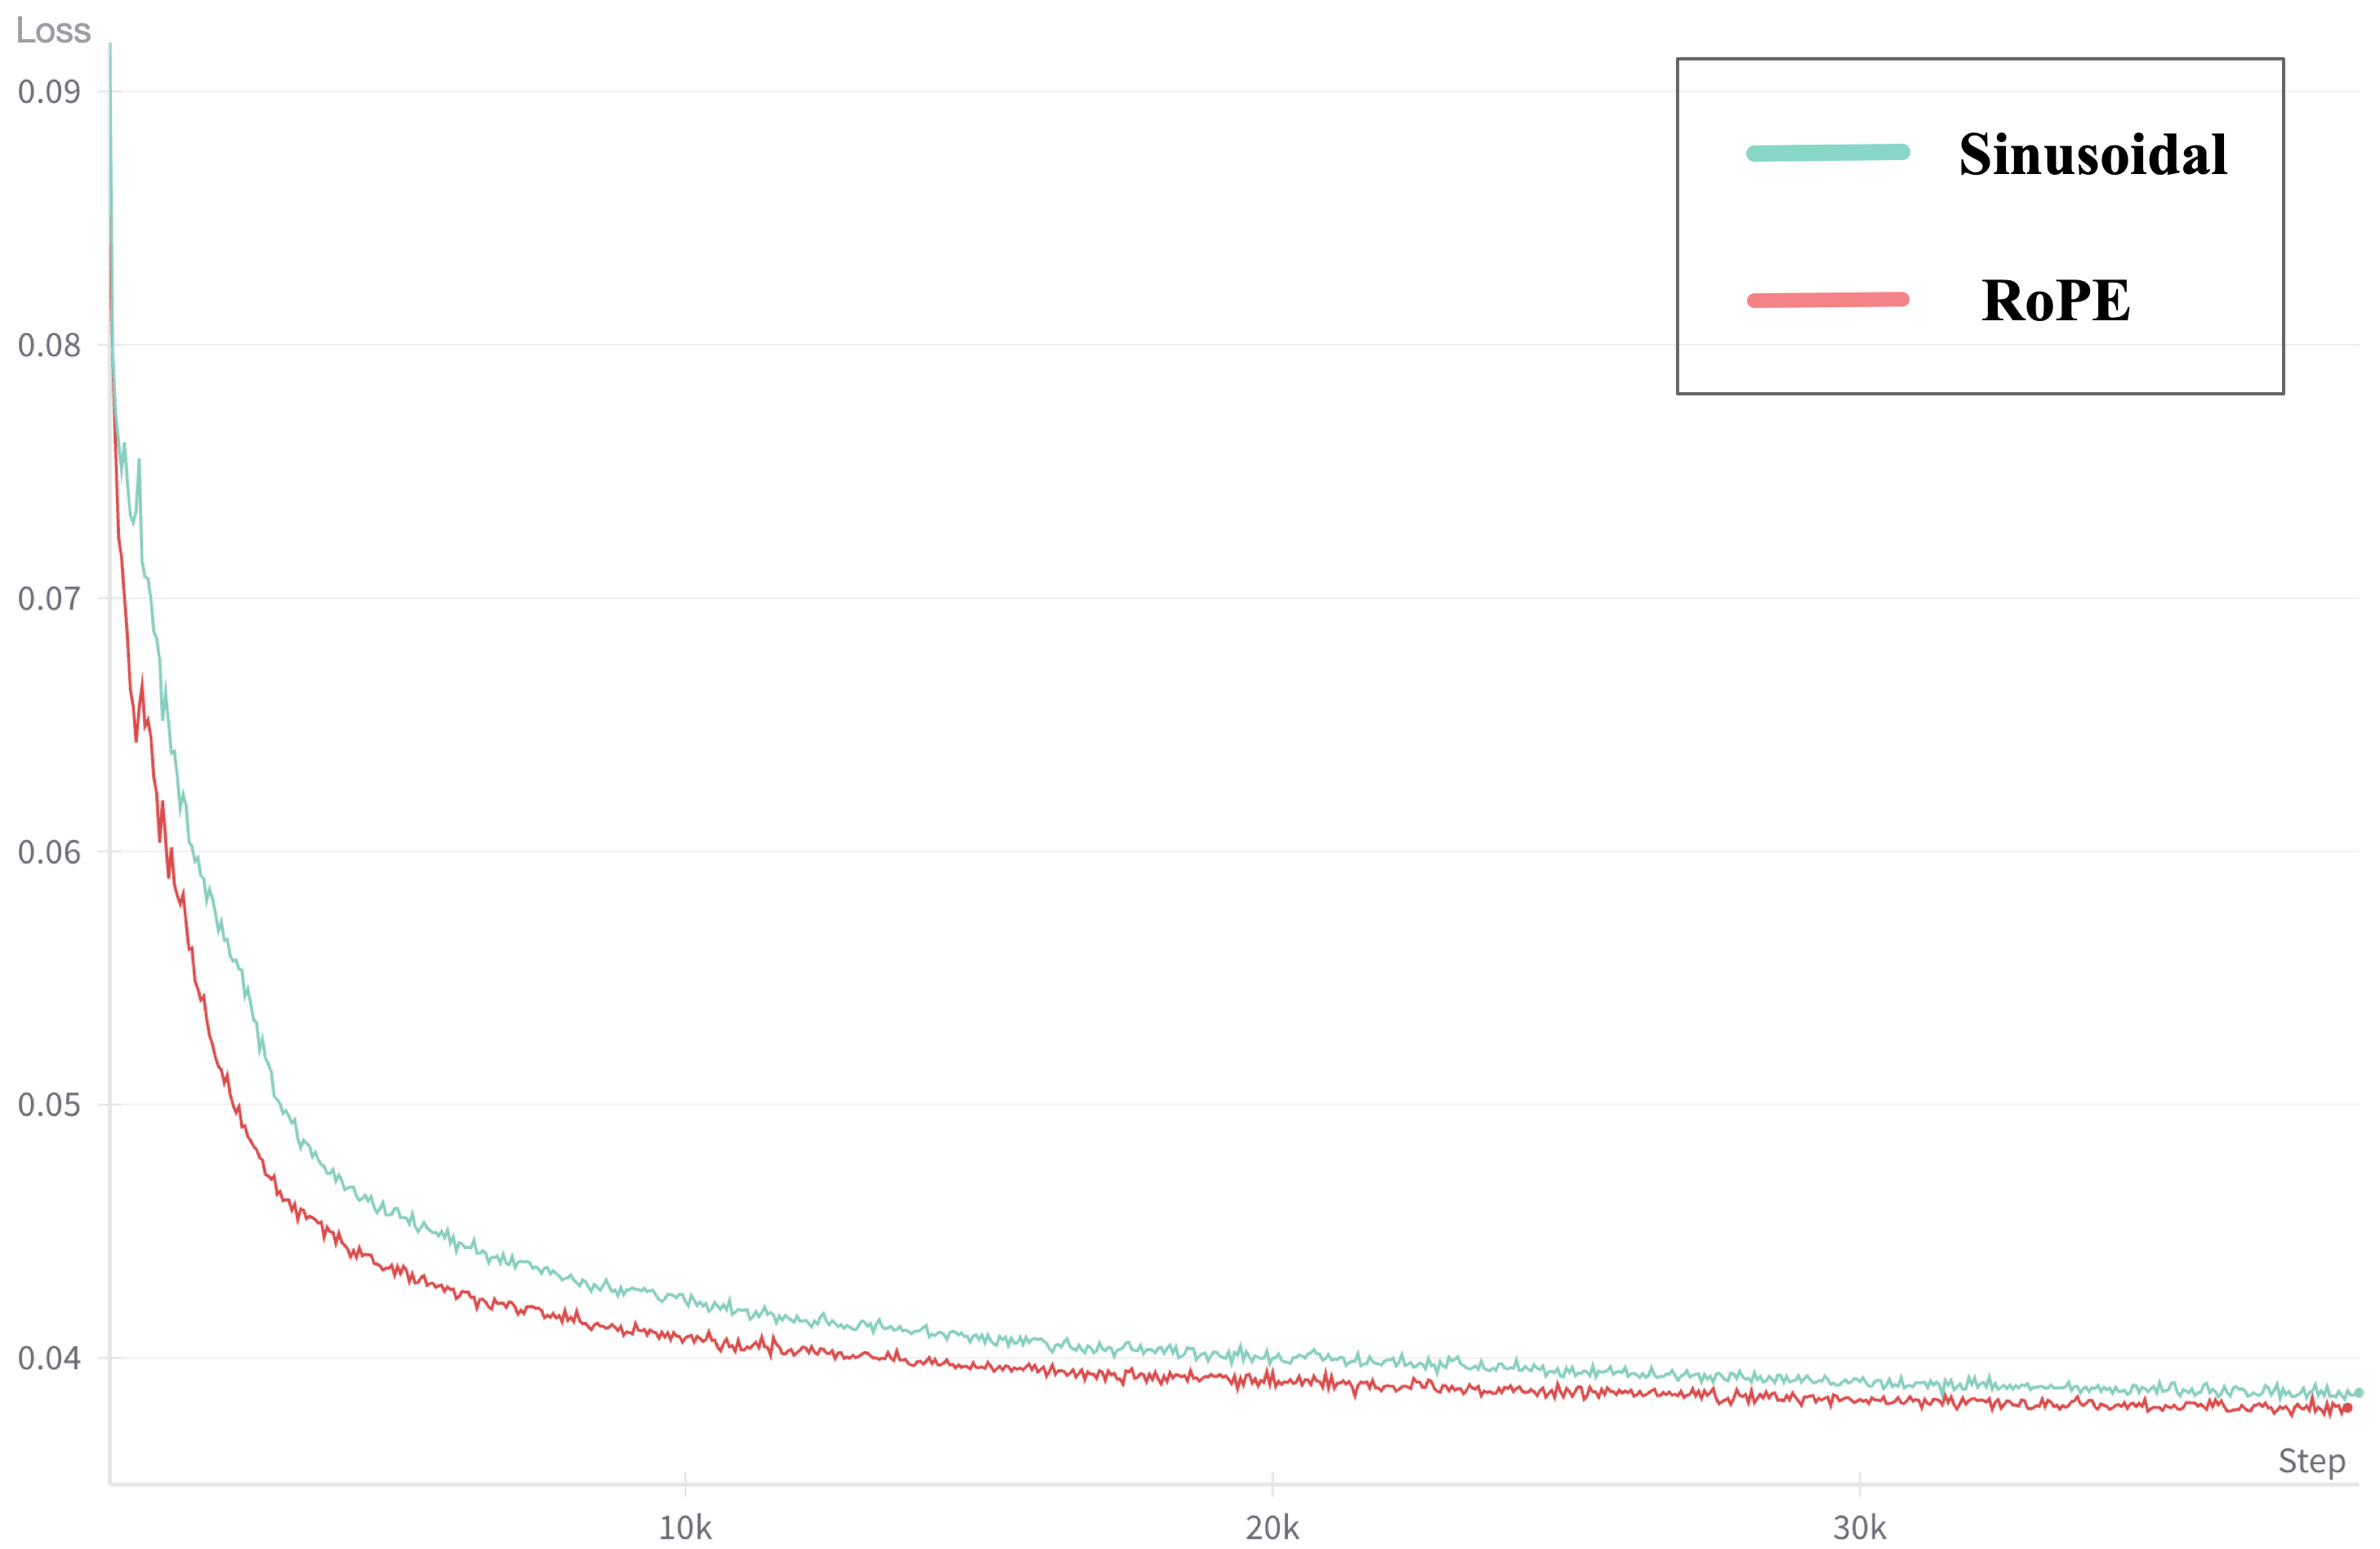
\includegraphics[width=\textwidth]{images/ab_sr.png}
%         \caption{RoPE vs. Sinusoidal}
%         \label{fig:rope-sin}
%     \end{subfigure}
%     \begin{subfigure}[b]{0.48\textwidth}
%         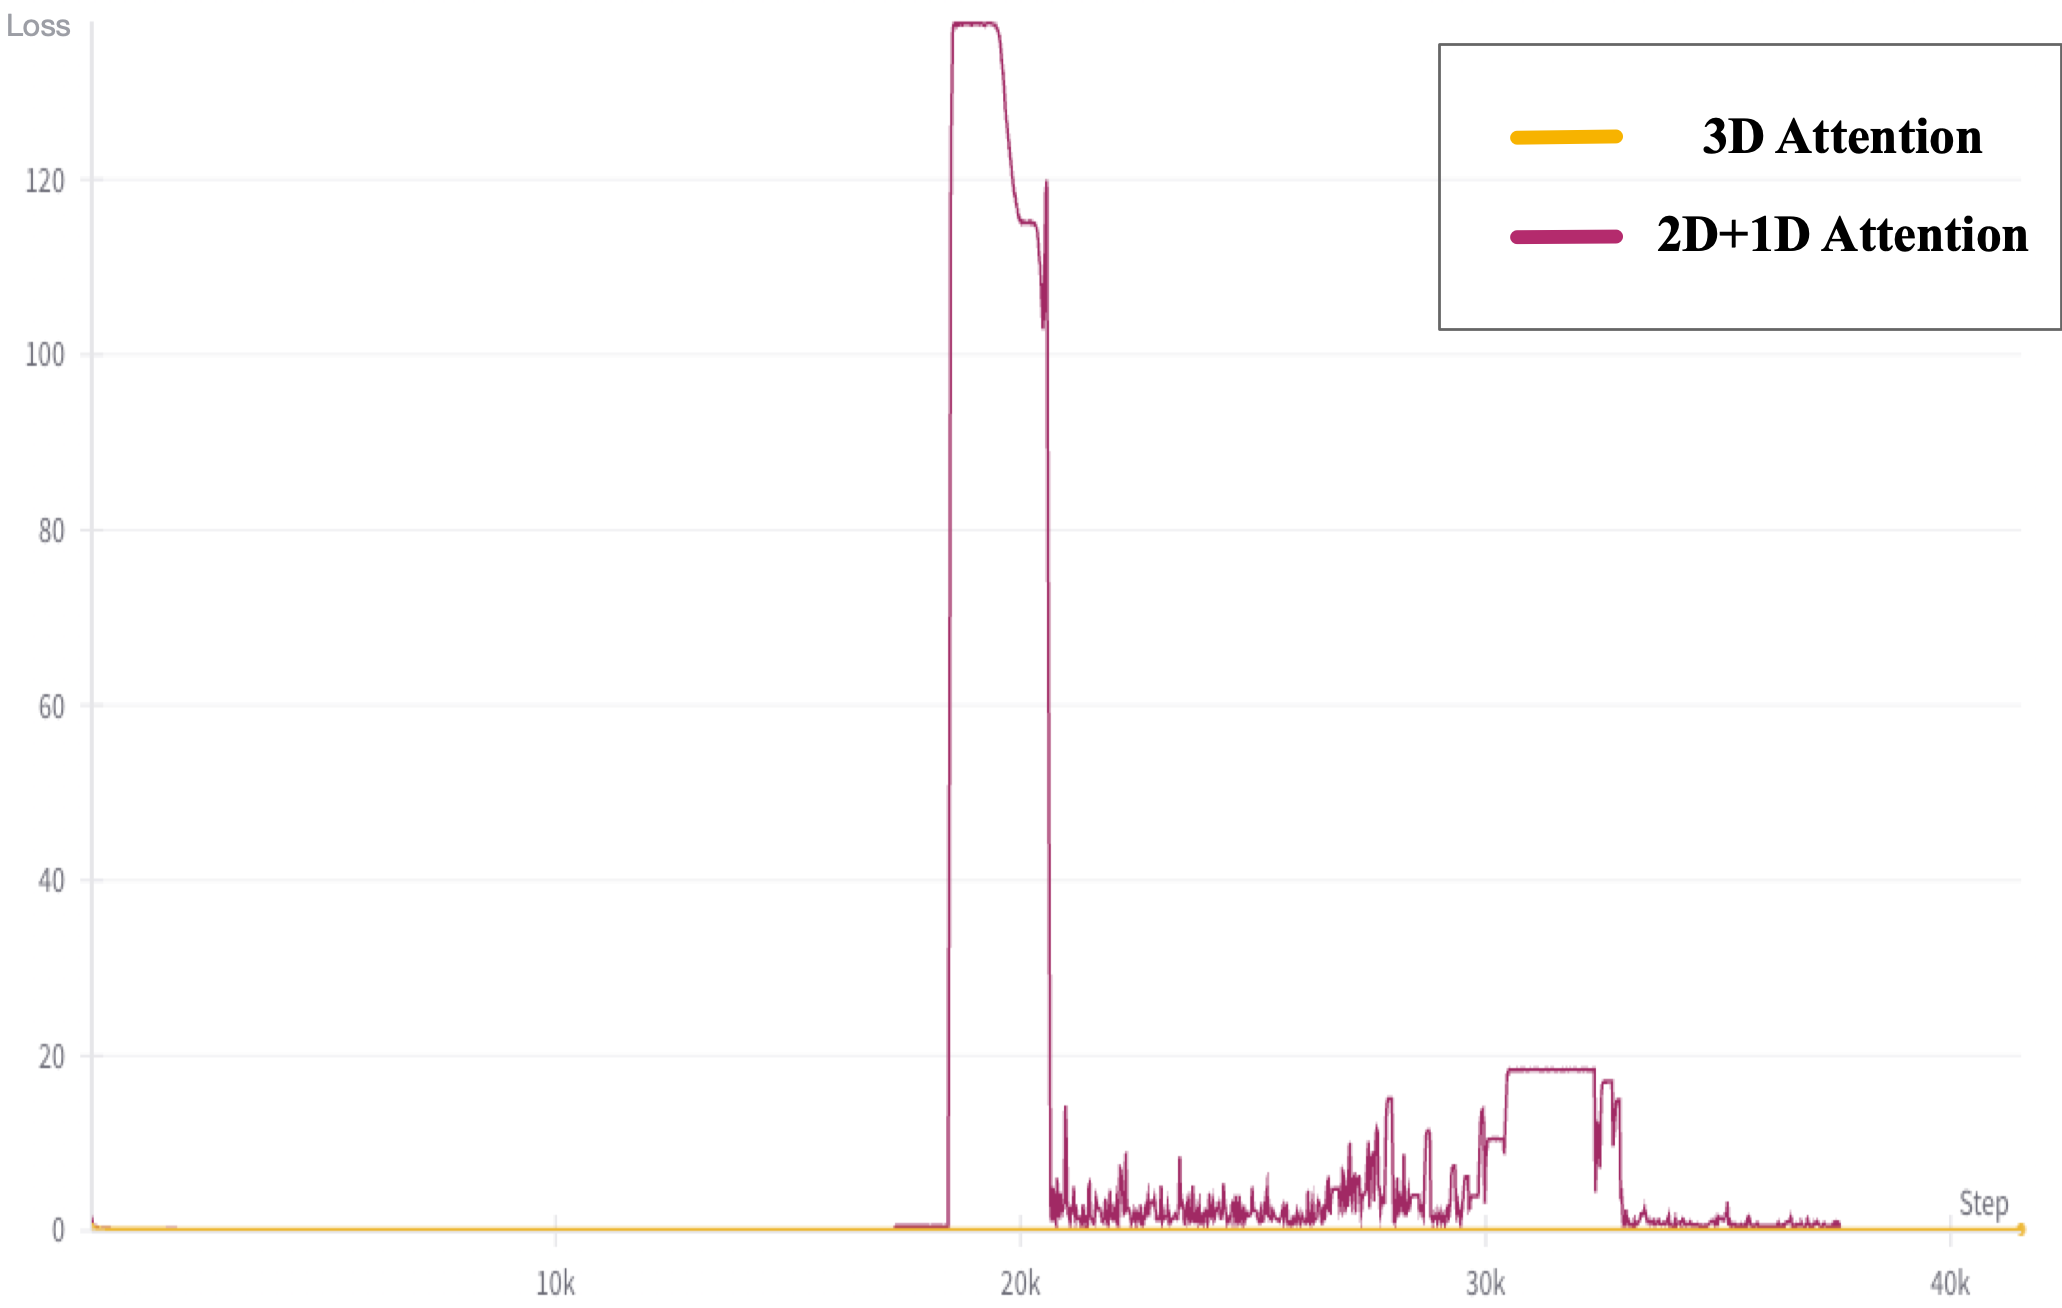
\includegraphics[width=\textwidth]{images/ab_rl.png}
%         \caption{RoPE vs. RoPE + Learnable}
%         \label{fig:rope-learnable}
%     \end{subfigure}
%     \begin{subfigure}[b]{0.46\textwidth}
%         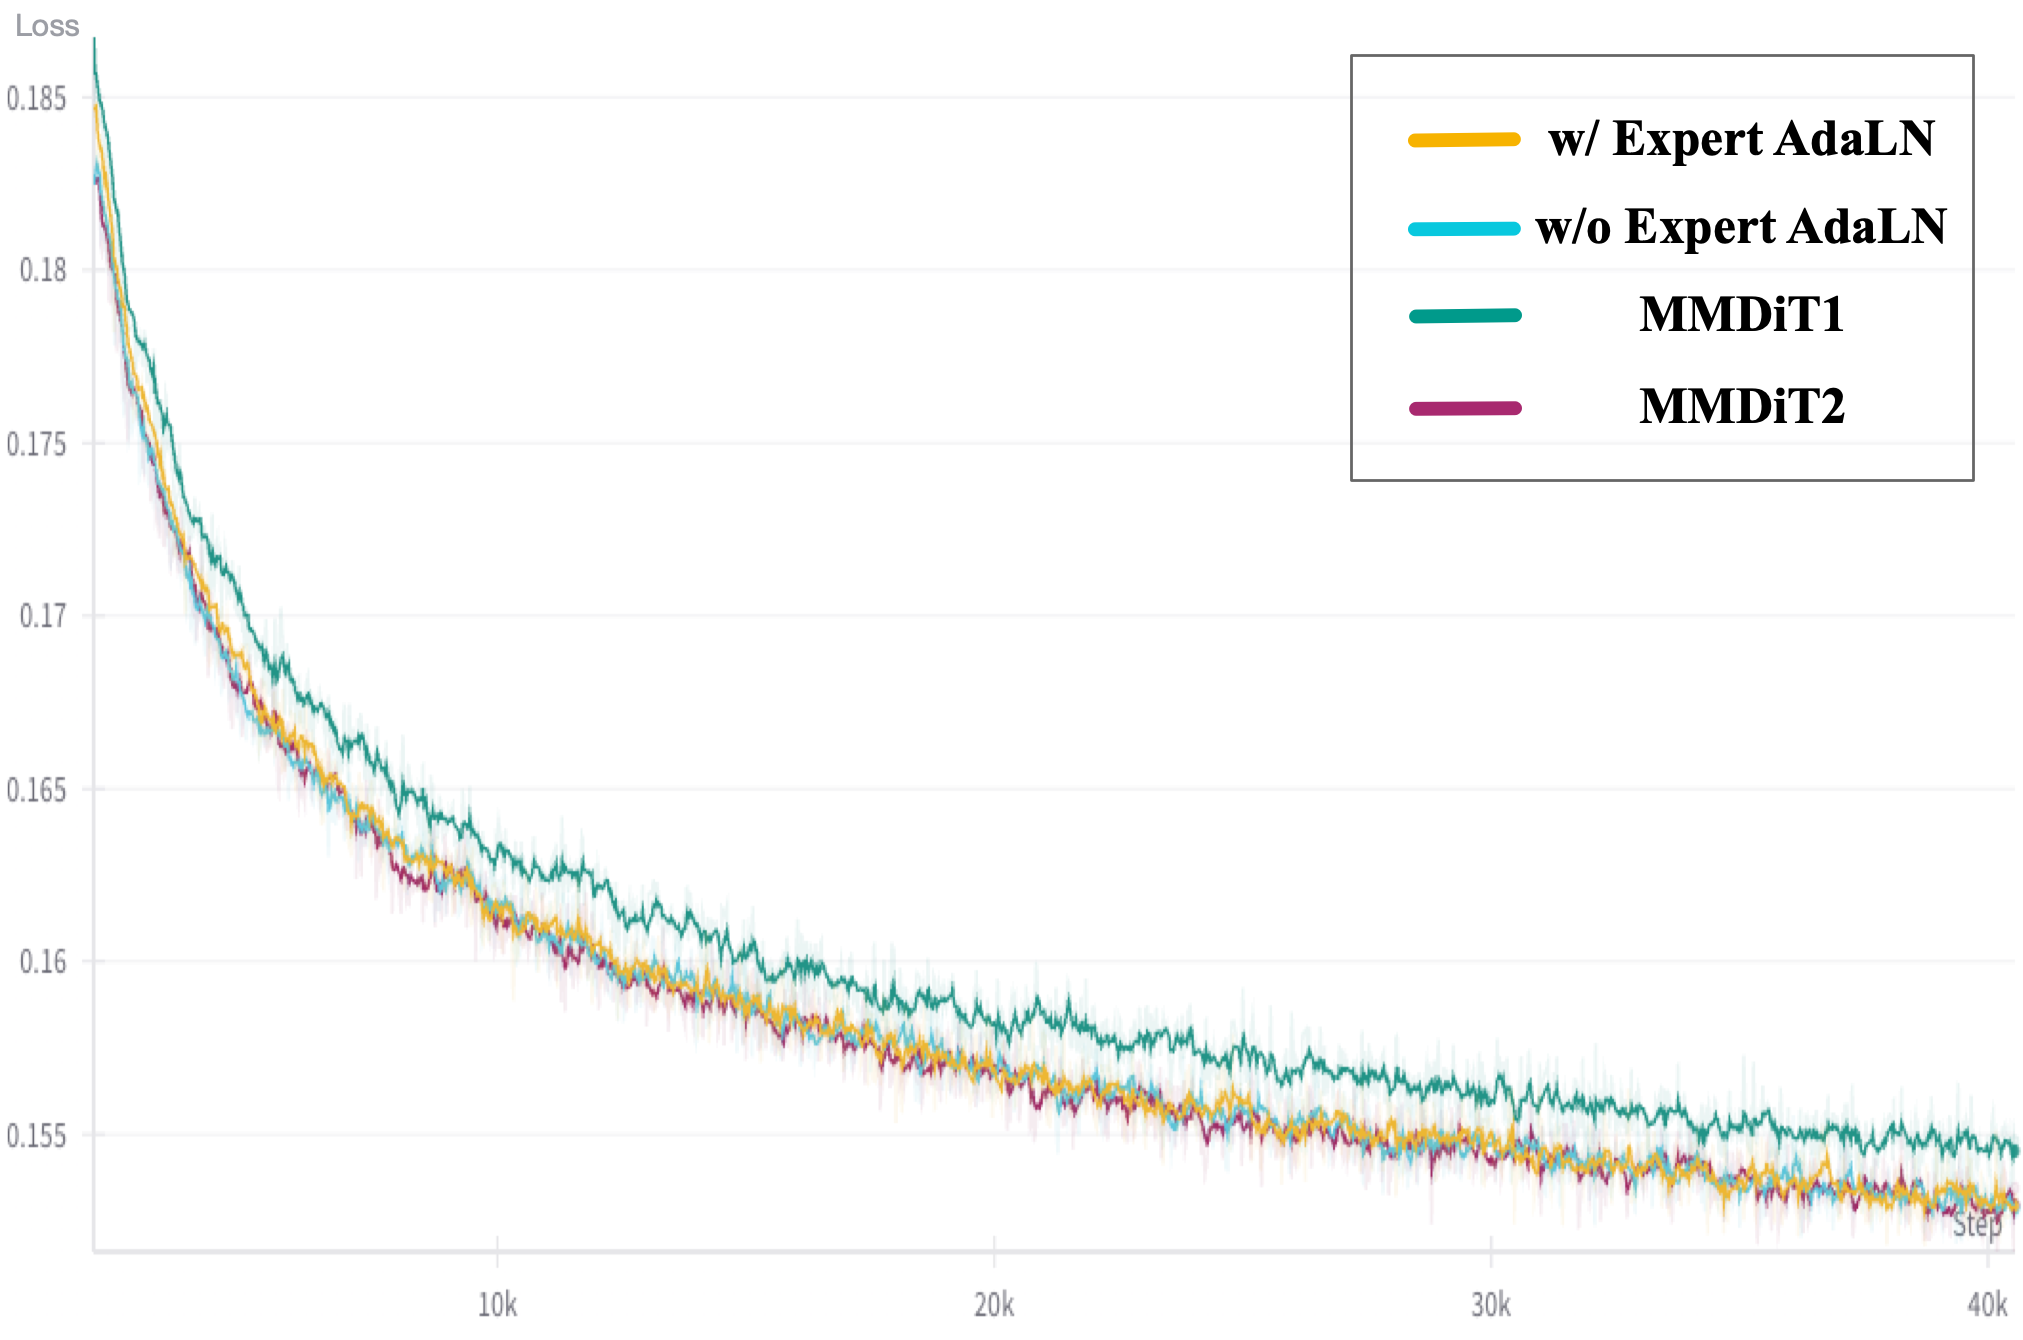
\includegraphics[width=\textwidth]{images/ab_ex.png}
%         \caption{Expert Ada. LN vs. Expert Ada. LN + MLP}
%         \label{fig:expert}
%     \end{subfigure}
%     \begin{subfigure}[b]{0.48\textwidth}
%         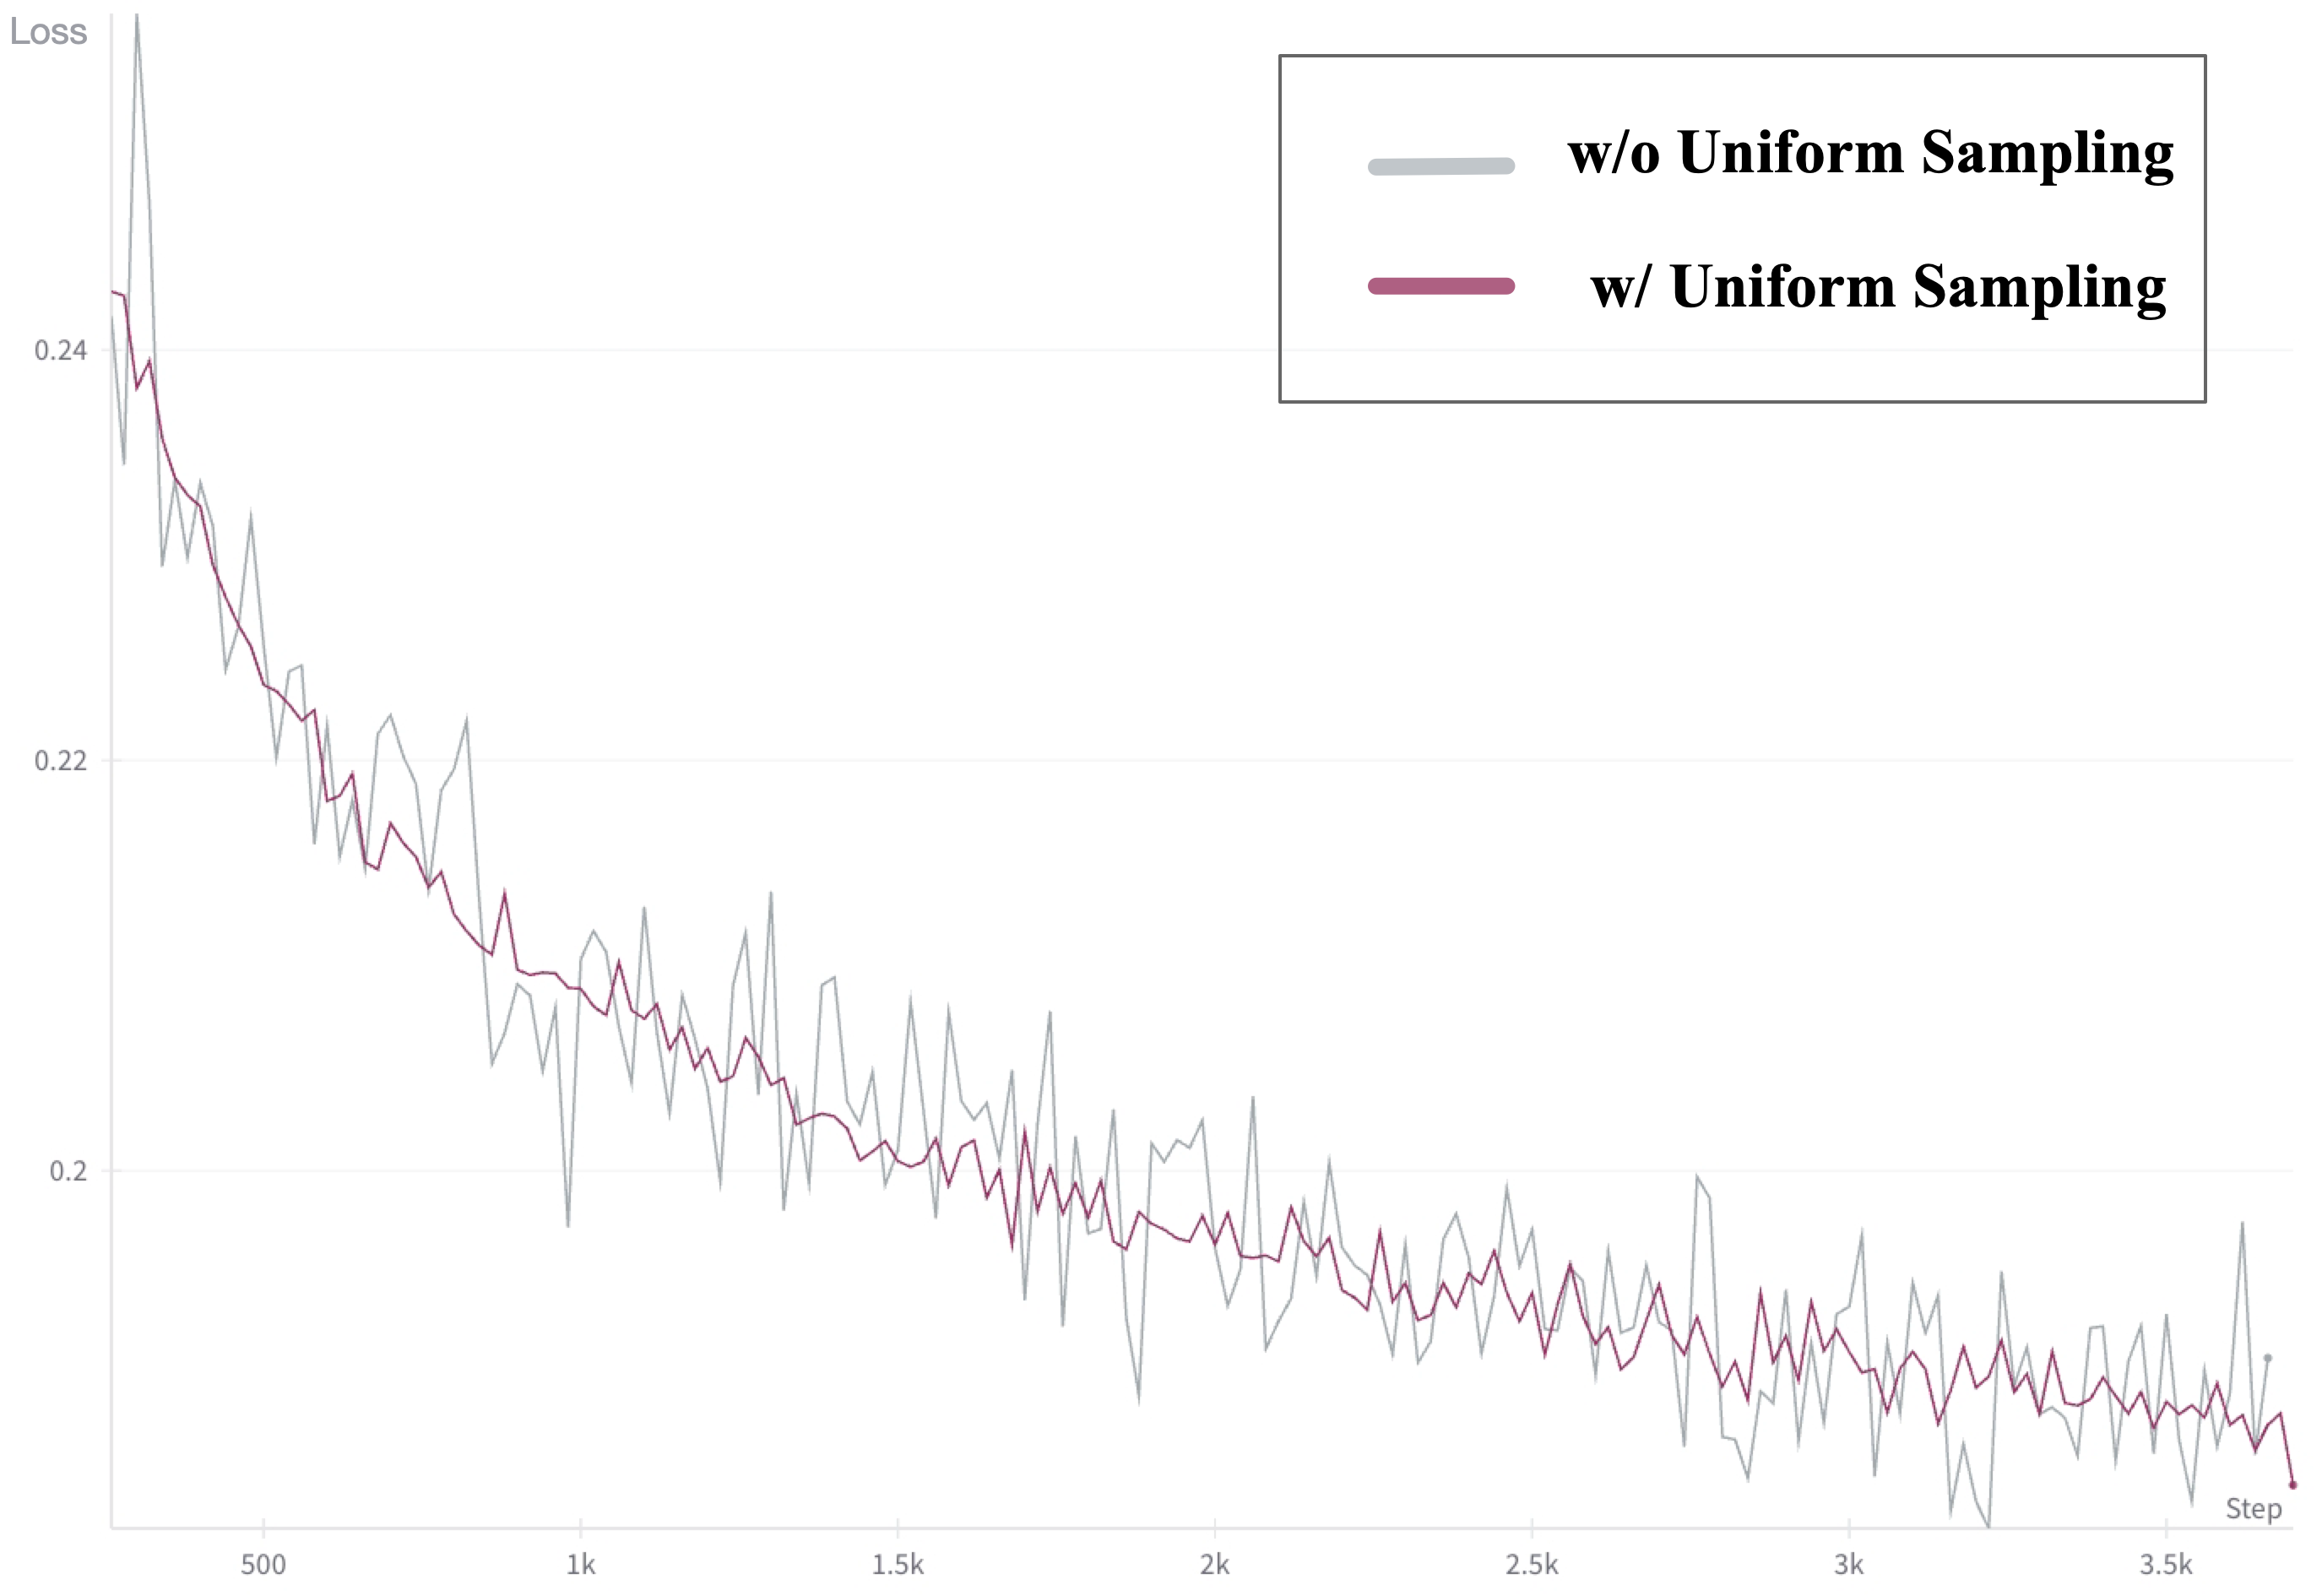
\includegraphics[width=\textwidth]{images/ab_us.png}
%         \caption{Uniform Sampling vs. No Uniform Sampling}
%         \label{fig:uniform-sampling}
%     \end{subfigure}

%     \caption{Training loss curve of different ablations.}
%     \label{fig:subfigures}
% \end{figure}

\begin{wrapfigure}{r}{0.5\textwidth}
% \begin{figure}[h]
\centering
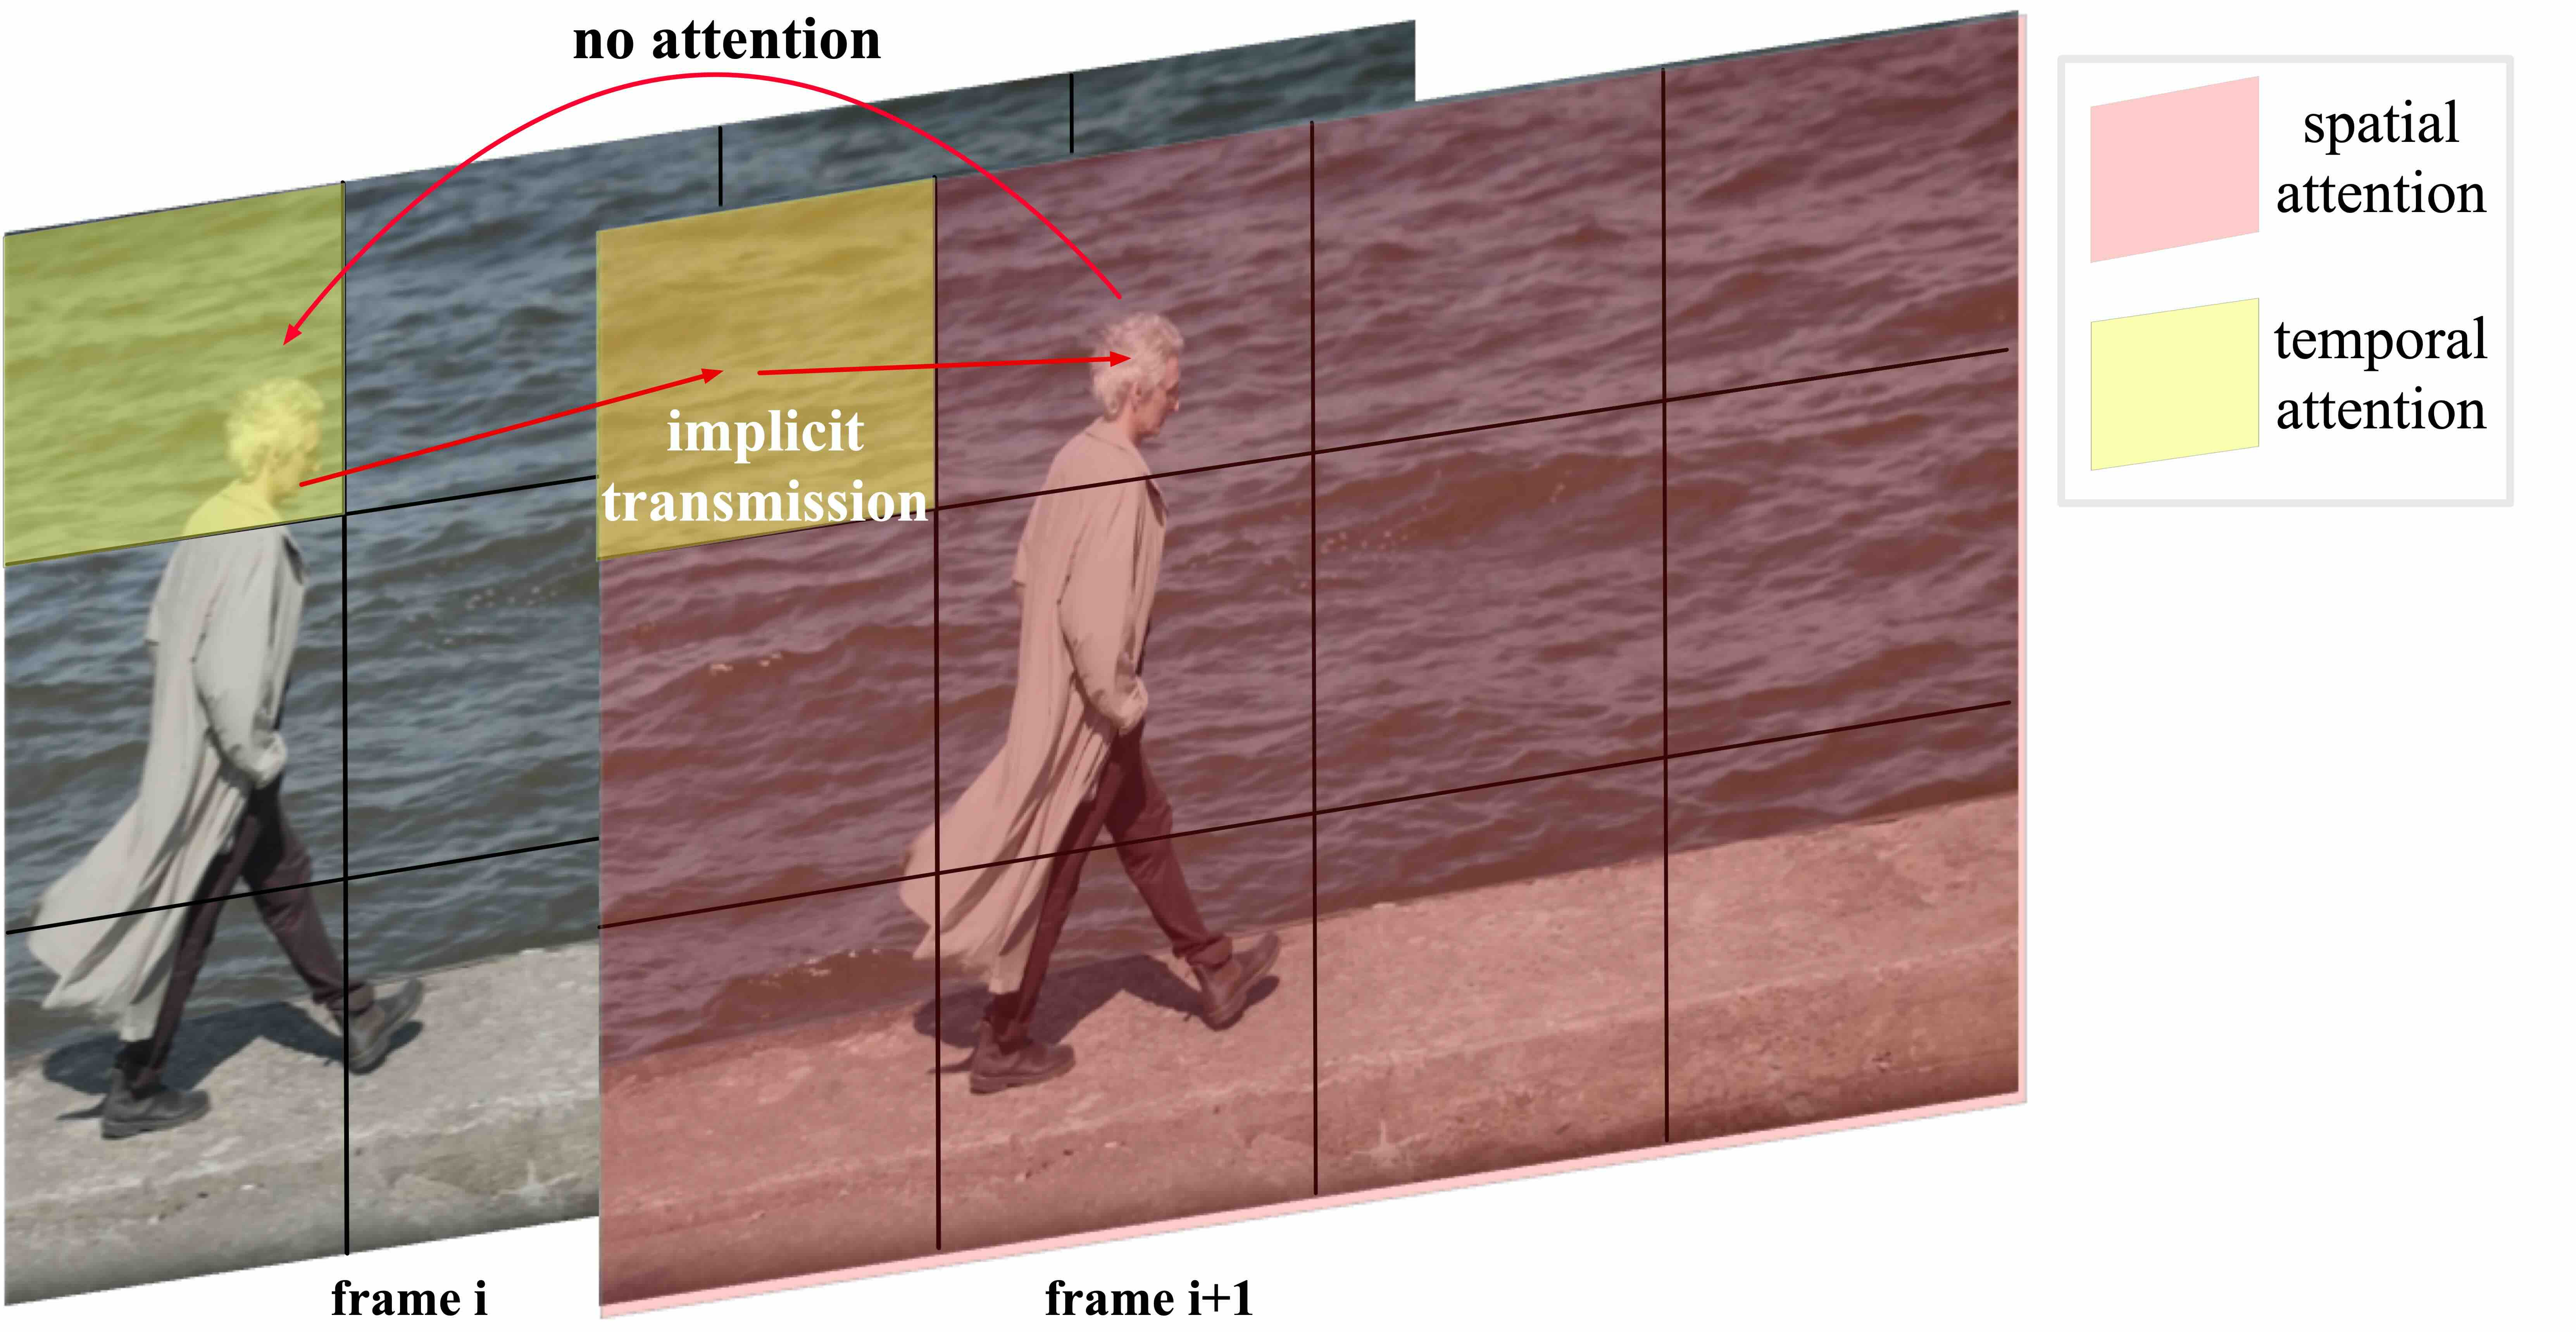
\includegraphics[width=\linewidth]{images/attention.jpg}
\caption{The separated spatial and temporal attention makes it challenging to  handle the large motion between adjacent frames. 
In the figure, the head of the person in frame $i+1$ cannot directly attend to the head in frame $i$. 
Instead, visual information can only be implicitly transmitted through other background patches. 
This can lead to inconsistency issues in the generated videos.}
\label{fig:attention}
%\vspace{-10mm}
% \end{figure}
\end{wrapfigure}


\paragraph{Expert Adaptive Layernorm.}
We concatenate the embeddings of both text and video at the input stage to better align visual and semantic information. 
However, the feature spaces of these two modalities differ significantly, and their embeddings may even have different numerical scales. 
To better process them within the same sequence, we employ the Expert Adaptive Layernorm to handle each modality independently.
As shown in Figure~\ref{fig:model}, following DiT~\citep{peebles2023scalable}, we use the timestep $t$ of the diffusion process as the input to the modulation module. 
Then, the Vision Expert Adaptive Layernorm (Vison Expert AdaLN) and Text Expert Adaptive Layernorm (Text Expert AdaLN) apply this modulation mechanism to the vision hidden states and text hidden states, respectively. 
This strategy promotes the alignment of feature spaces across two modalities while minimizing additional parameters.

% To verify the adoption of Expert Adaptive Layernorm, we experiment with different ways of incorporating experts: expert LayerNorm and MLP, and expert Layernorm only. 
% Our experiments find that adding expert MLP does not effectively accelerate the model's convergence (Cf. Figure~\ref{fig:subfigures} (c)). 
% To reduce the model parameters, we only choose to use Expert Adaptive Layernorm.



\paragraph{3D Full Attention.}
Previous works \citep{singer2022make, guo2023animatediff} often employ separated spatial and temporal attention to reduce computational complexity and facilitate fine-tuning from text-to-image models. 
However, as illustrated in Figure~\ref{fig:attention}, this separated attention approach requires extensive implicit transmission of visual information, significantly increasing the learning complexity and making it challenging to maintain the consistency of large-movement objects. 
Considering the great success of long-context training in LLMs~\citep{llama3modelcard}  and the efficiency of FlashAttention~\citep{dao2022flashattention},  we propose a 3D text-video hybrid attention mechanism. 
This mechanism not only achieves better results but can also be easily adapted to various parallel acceleration methods. 


\hide{
\begin{wrapfigure}{r}{0.5\textwidth}
\centering
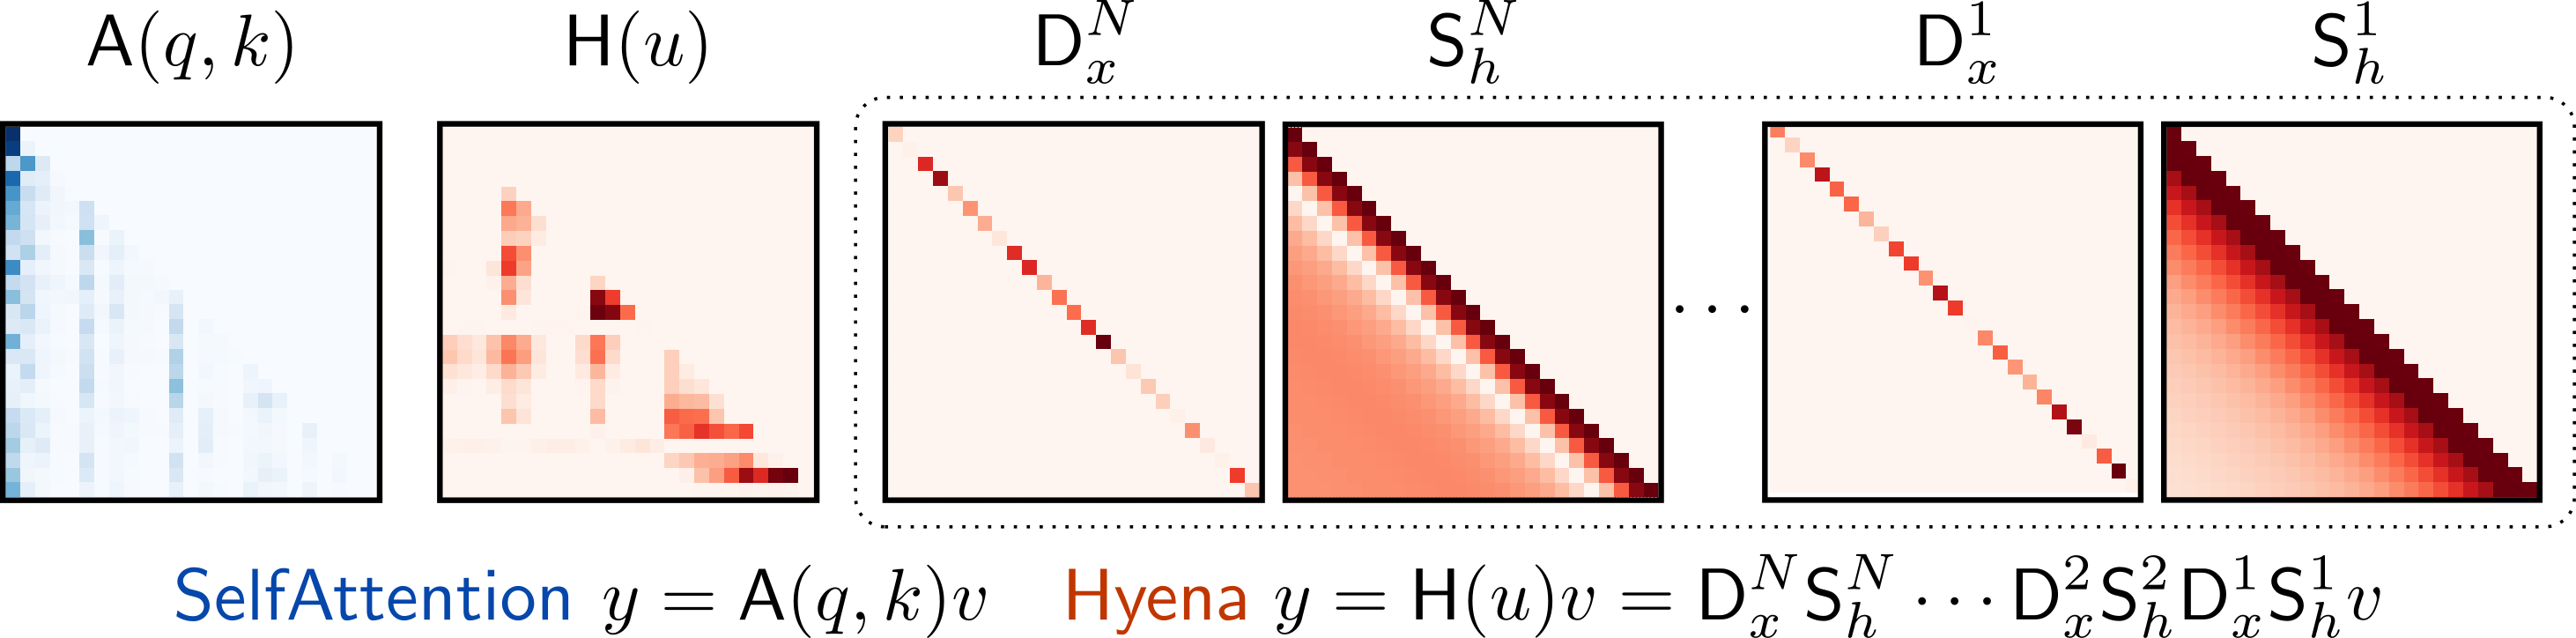
\includegraphics[width=\linewidth]{images/attention.png}
\caption{The separated spatial and temporal attention makes it challenging to handle the large motion between adjacent frames. In the figure, the head of the person in frame $i+1$ cannot directly attend to the head in the frame $i$. Instead, visual information can only be implicitly transmitted through other background patches. This can lead to inconsistency issues in the generated videos.}
\label{fig:attention}
\vspace{-10mm}
\end{wrapfigure}
}%end of hide



